%&LaTeX
% !TEX encoding = UTF-8 Unicode
\documentclass{report}
\usepackage[utf8]{inputenc}
\usepackage[T1]{fontenc}
\usepackage{textcomp}
\usepackage{float,fancyvrb}
\usepackage{listings}

%\usepackage{graphicx}
\usepackage{longtable}
\usepackage{color}

\usepackage{ifpdf}

\ifx\pdftexversion\undefined %if using TeX
    \usepackage{graphicx}
\else %if using PDFTeX
    \ifpdf %if using PDFTeX in PDF mode
        \usepackage[pdftex]{graphicx}
        \DeclareGraphicsExtensions{.pdf,.png,.mps}
        \usepackage{pgf}
    \else %if using TeX or PDFTeX in TeX mode
        \usepackage{graphicx}
        \DeclareGraphicsExtensions{.eps,.bmp}
        \DeclareGraphicsRule{.emf}{bmp}{}{}% declare EMF filename extension
        \DeclareGraphicsRule{.png}{bmp}{}{}% declare PNG filename extension
        \usepackage{pgf}
        \usepackage{pstricks} %variant: \usepackage{pst-all}
\fi

%\setlength{\paperheight}{297mm}
%\setlength{\paperwidth}{210mm}
%\setlength{\voffset}{11mm}
\setlength{\topmargin}{0mm}
\setlength{\headsep}{0mm}
\setlength{\headheight}{0mm}
\setlength{\textheight}{235mm}
\setlength{\hoffset}{-4mm}
\setlength{\textwidth}{166mm}
\setlength{\oddsidemargin}{0mm}
\setlength{\evensidemargin}{0mm}
\setlength{\marginparwidth}{0mm}
\setlength{\marginparpush}{0mm}
%\setlength{\columnsep}{6mm}
%\setlength{\parindent}{0mm}


\definecolor{color01}{rgb}{0.00,0.00,0.00}
\definecolor{color02}{rgb}{0.00,0.00,1.00}
\definecolor{color06}{rgb}{1.00,0.00,0.00}
\definecolor{color08}{rgb}{1.00,1.00,1.00}
\definecolor{color17}{rgb}{0.14,0.25,0.38}
\definecolor{color20}{rgb}{0.31,0.51,0.74}
\definecolor{color26}{rgb}{0.50,0.50,0.50}

%% Added by Jong -- to enable \subsubsection
\setcounter{secnumdepth}{3}
\usepackage{hyperref}

\newcommand{\comment}[1]{}
\newcommand{\adiosversion}{ADIOS 1.6\xspace}

%%%%%%%%%%%%%%%%%%%%%%%%%%%%%%%%%%%%%%%%%%%%%%%%%%%%%%%%%%%%%%%%%%%%%%%
% Define syntax highlighting for ADIOS
\lstdefinelanguage{ADIOS}
{
sensitive=true,
keywordsprefix=ADIOS_,
morekeywords=[1]{
adios_errno, err_file_not_found, err_end_of_stream, err_step_notready, err_step_deleted},
morekeywords=[2]{
% Write API (XML)
adios_init, adios_finalize, adios_open, adios_write, adios_read, adios_close, 
adios_group_size, adios_set_path_var, adios_set_path, 
adios_end_iteration, adios_start_calculation, adios_stop_calculation,
% Write API (Non-XML)
adios_init_noxml, adios_declare_group, adios_free_group, adios_define_var, 
adios_define_attribute, adios_allocate_buffer, adios_select_method,
adios_get_write_buffer,
% Read API (1.4)
adios_read_init_method, adios_read_finalize_method,
adios_read_open_file, adios_read_open, adios_read_close,
adios_inq_var, adios_inq_var_byid, adios_free_varinfo,
adios_inq_var_stat, adios_inq_var_blockinfo,
adios_get_attr, adios_get_attr_byid,
adios_schedule_read, adios_schedule_read_byid, adios_perform_reads, adios_check_reads,
adios_advance_step, adios_release_step,adios_free_chunk,
adios_selection_boundingbox, adios_selection_points, adios_selection_writeblock, 
adios_selection_delete, adios_selection_auto, adios_errmsg,
adios_type_to_string, adios_type_size, adios_get_grouplist,
% Fortran Read
adios_reset_dimension_order, adios_inq_ngroups, adios_inq_groupnames, 
adios_group_view, adios_inq_file, adios_inq_varnames, adios_inq_attrnames,
adios_inq_attr, adios_get_scalar, adios_get_statistics},
morecomment=[l]{//},morecomment=[s]{/*}{*/},
morestring=[b]",morestring=[b]',
}

\lstdefinelanguage{cython}[]{python}
{
sensitive=true,
keywordsprefix=ADIOS_,
keywords={def, cpdef, cdef, public, class, self},
morekeywords=[1]{
int64_t, uint64_t, int, long, float, double, char, bytes, tuple, list, dict},
upquote=true,
}

\lstdefinelanguage{ADIOS-python}[]{python}
{
upquote=true,
}

\definecolor{gray}{rgb}{0.35,0.35,0.35}
\definecolor{gray85}{rgb}{0.85,0.85,0.85}
\definecolor{javared}{rgb}{0.6,0,0}
\definecolor{javagreen}{rgb}{0.25,0.5,0.35}
\definecolor{javapurple}{rgb}{0.5,0,0.35}
\definecolor{javadocblue}{rgb}{0.25,0.35,0.75}

\lstset{language=ADIOS, basicstyle=\ttfamily, numbers=none,
  showspaces=false, showstringspaces=false,
  keywordstyle=[1]\color{javapurple},
  keywordstyle=[2]\color{blue}\bf,
  stringstyle=\color{javared},
  commentstyle=\color{javagreen},
  captionpos=b,
  frame=no,
  escapechar=`,
}
% End of syntax highlight def for ADIOS
%%%%%%%%%%%%%%%%%%%%%%%%%%%%%%%%%%%%%%%%%%%%%%%%%%%%%%%%%%%%%%%%%%%%%%%

\begin{document}


\vspace{24pt}
\begin{flushright}
{\color{color08} \textbf{ORNL/TM-2009/100\label{OLEHLINK6}}}
\end{flushright}

\vspace{60pt}
{\huge \textbf{ADIOS 1.6.0 Developer's Manual}}

\vspace{36pt}
\textbf{December 2013\pagebreak{}}


\begin{longtable}{|p{4.443in}|p{0.057in}|}
\hline

\begin{center}
{\small \textbf{DOCUMENT AVAILABILITY}}
\end{center}


{\small Reports produced after January 1, 1996, are generally available free via 
the U.S. Department of Energy (DOE) Information Bridge:}


\leftskip=18pt
{\small \textbf{Web site:}}{\small  http://www.osti.gov/bridge}


\leftskip=0pt
{\small Reports produced before January 1, 1996, may be purchased by members of 
the public from the following source:}


\parindent=18pt
{\small National Technical Information Service}

{\small 5285 Port Royal Road}

{\small Springfield, VA 22161}

{\small \textit{\textbf{Telephone:}}}{\small  703-605-6000 (1-800-553-6847)}

{\small \textit{\textbf{TDD:}}}{\small  703-487-4639}

{\small \textit{\textbf{Fax:}}}{\small  703-605-6900}

{\small \textit{\textbf{E-mail:}}}{\small  info@ntis.fedworld.gov}

{\small \textit{\textbf{Web site:}}}{\small  http://www.ntis.gov/support/ordernowabout.htm}


\parindent=0pt
{\small Reports are available to DOE employees, DOE contractors, Energy Technology 
Data Exchange (ETDE) representatives, and International Nuclear Information System 
(INIS) representatives from the following source:}


\parindent=18pt
{\small Office of Scientific and Technical Information}

{\small P.O. Box 62}

{\small Oak Ridge, TN 37831}

{\small \textit{\textbf{Telephone:}}}{\small  865-576-8401}

{\small \textit{\textbf{Fax:}}}{\small  865-576-5728}

{\small \textit{\textbf{E-mail:}}}{\small  reports@adonis.osti.gov}

\leftskip=18pt
\parindent=0pt
{\small \textit{\textbf{Web site:}}}{\small  http://www.osti.gov/contact.html}

\\\hline
\end{longtable}

%\vspace{48pt}
\begin{longtable}{|p{4.443in}|p{0.057in}|}
\hline
% ROW 1
\begin{minipage}[t]{4.443in}\raggedright %\linebreak
{\small This report was prepared as an account of work sponsored by an agency of 
the United States Government. Neither the United States government nor any agency 
thereof, nor any of their employees, makes any warranty, express or implied, or 
assumes any legal liability or responsibility for the accuracy, completeness, or 
usefulness of any information, apparatus, product, or process disclosed, or represents 
that its use would not infringe privately owned rights. Reference herein to any 
specific commercial product, process, or service by trade name, trademark, manufacturer, 
or otherwise, does not necessarily constitute or imply its endorsement, recommendation, 
or favoring by the United States Government or any agency thereof. The views and 
opinions of authors expressed herein do not necessarily state or reflect those 
of the United States Government or any agency thereof.}\end{minipage}\\
\hline
\end{longtable}
\pagebreak{}

\vspace{12pt}
\begin{flushright}
{\color{color08} \textbf{ORNL/TM-2009/100\label{HToc533553247}\label{HToc6041549}\label{HToc6042388}\label{HToc8548020}\label{HToc528144461}\label{HToc528743868}\label{HToc528745033}}}
\end{flushright}

%\vspace{36pt}
\begin{center}
{\Large \textbf{ADIOS 1.6.0 DEVELOPER'S MANUAL}}

\vspace{60pt}
Prepared for the

%\vspace{12pt}
Office of Science

%\vspace{12pt}
U.S. Department of Energy

\vspace{60pt}
Authors

\vspace{6pt}
N. Podhorszki, Q. Liu, J. Logan, H. Abbasi, J.Y. Choi, S. Klasky

\vspace{30pt}
Contributors 

\vspace{6pt}
J. Lofstead, S. Hodson, F. Zheng, M. Wolf, T. Kordenbrock, N. Samatova, J.Q. Mu, J. Dayal, Y. Tian

\vspace{72pt}
December 2013

\vspace{72pt}
Prepared by

%\vspace{24pt}
OAK RIDGE NATIONAL LABORATORY

%\vspace{12pt}
Oak Ridge, Tennessee 37831-6070

%\vspace{12pt}
managed by

%\vspace{12pt}
UT-BATTELLE, LLC

%\vspace{12pt}
for the

%\vspace{12pt}
U.S. DEPARTMENT OF ENERGY

%\vspace{12pt}
under contract DE-AC05-00OR22725

%\vspace{42pt}
\end{center}


\newpage

\tableofcontents


\newpage

\listoffigures


\newpage


\vspace{66pt}
\textbf{Abbreviations}

\begin{description}
\item[ADIOS]  Adaptive Input/Output System
\item[API] Application Program Interface
\item[DART] Decoupled and Asynchronous Remote Transfers
\item[GTC] Gyrokinetic Turbulence Code
\item[HPC] High-Performance Computing
\item[I/O] Input/Output
\item[MDS] Metadata Server
\item[MPI] Message Passing Interface
\item[NCCS] National Center for Computational Sciences
\item[ORNL] Oak Ridge National Laboratory
\item[OS] Operating System
\item[PG] Process Group
\item[POSIX] Portable Operating System Interface
\item[RDMA] Remote Direct Memory Access
\item[XML] Extensible Markup Language
\end{description}


\vspace{18pt}
\begin{center}
{\large \textbf{Acknowledgments}}
\end{center}

\vspace{6pt}
This project is sponsored by ORNL, Georgia Tech, The Scientific Data Management 
Center (SDM) at Lawrence Berkeley National Laboratory, and the U.S. Department 
of Defense. 



\chapter{Introduction}

Skel is a tool used for the generation of I/O skeletal applications. Skel takes a
high-level description of the I/O performed by an application, and generates a full
benchmark that performs the described I/O.
Compared to a scientific application, the generated benchmark is easy to build
and run, and generally runs faster since it only performs I/O. Despite
the simplicity of the generated code, it duplicates
the I/O pattern of the target application, thus simplifying the process of
understanding the I/O performance of an application.

Skel provides a simple mechanism for testing the performance of I/O operations
that are relevant to applications of interest. This is of critical importance
when evaluating new systems or new system configurations. It is equally useful
for evaluating new I/O methods, or examining the effects of dirent parameters
to existing I/O methods. Since the benchmarks produced by skel focus
on the exact I/O patterns of applications, performance measurements obtained
from those benchmarks will correlate highly with the performance of the actual
applications.

This manual provides a detailed explanation of Skel, including the relevant
file formats, documentation of skel commands, common usage of skel, and hints
for porting skel to new platforms. Skel is young and still in development, so we
expect there will be things that do not work perfectly, as well as things that 
have changed from the previous release. Please help us improve by
letting us know when you encounter troubles. You can reach the skel developers
by sending email to lot@ornl.gov.



\chapter{BP File Format}

\section{Introduction}

This chapter describes the file structure of BP, which is the ADIOS native binary 
file format, to aid in understanding ADIOS performance issues and how files convert 
from BP files to other scientific file formats, such as netCDF and HDF5.

To avoid the file size limitation of 2 gigabytes by using a signed 32-bit offset 
within its internal structure, BP format uses an unsigned 64-bit datatype as the 
file offset. Therefore, it is possible to write BP files that exceed 2 gigabytes 
on platforms that have large file support. 

By adapting ADIOS read routines based on the endianness indication in the file 
footer, BP files can be easily portable across different machines (e.g., between 
the Cray-XT4 and BlueGene). 

To aid in data selection, we have a low-overhead concept of data characteristics 
to provide an efficient, inexpensive set of attributes that can be used to identify 
data sets without analyzing large data content.

As shown in Figure \ref{fig:bp-file-struct}, 
the BP format comprises a series of process groups and the 
file footer. The remainder of this chapter describes each component in detail and 
helps the user to better understand (1) why BP is a self -describing and metadata-rich 
file format and (2) why it can achieve high I/O performance on different machine 
infrastructures. 

\begin{figure}[htbp]
\begin{center}
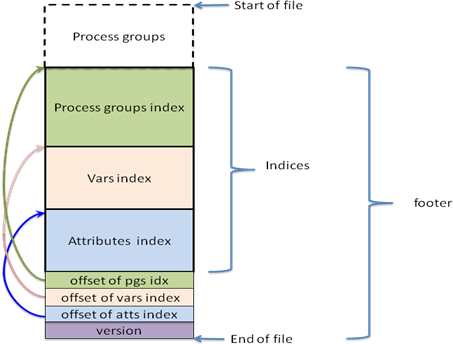
\includegraphics[width=217pt, height=163pt]{figures/bp-file-structure.png}
\caption{BP file structure}
\label{fig:bp-file-struct}
\end{center}
\end{figure}

\section{Footer}

One known limitation of the NetCDF format is that the file contents are stored 
in a header that is exactly big enough for the information provided at file creation. 
Any changes to the length of that data will require moving data. To avoid this 
cost, we choose to employ a foot index instead. We place our version identifier 
and the offset to the beginning of the index as the last few bytes of our file, 
making it simple to find the index information and to add new and different data 
to our files without affecting any data already written. 

\subsection{Version}

We reserve 4 bytes for the file version, in which the highest bit indicates endianness. 
Because ADIOS uses a fixed-size type for data, there is no need to store type size 
information in the footer. 

\subsection{Offsets of indices}

In BP format, we store three 8-byte file offsets right before the version word, 
which allows users or developers to quickly seek any of the index tables for process 
groups, variables, or attributes. 

\subsection{Indices}

\subsubsection{Characteristics}

Before we dive into the structures of the three index tables mentioned earlier, 
let's first take a look what characteristic means in terms of BP file format. To 
be able to make a summary inspection of the data to determine whether it contains 
the feature of greatest interest, we developed the idea of data characteristics. 
The idea of data characteristics is to collect some simple statistical and/or analytical 
data during the output operation or later for use in identifying the desired data 
sets. Simple statistics like array minimum and maximum values can be collected 
without extra overhead as part of the I/O operation. Other more complex analytical 
measures like standard deviations or specialized measures particular to the science 
being performance by require more processing. As part of our BP format, we store 
these values not only as part of data payload, but also in our index. 

\subsubsection{PG Index table}

As shown in Figure \ref{fig:group-index-table}, 
the process group (PG) index table encompasses the count 
and the total length of all the PGs as the first two entries. The rest of the tables 
contain a set of information for each PG, which contains the group name information, 
process ID, and time index. The Process ID specifies which process a group is written 
by. That process will be the rank value in the communicator if the MPI method is 
used. Most importantly, there is a file-offset entry for each PG, allowing a fast 
skip of the file in the unit of the process group.

\begin{figure}[htbp]
\begin{center}
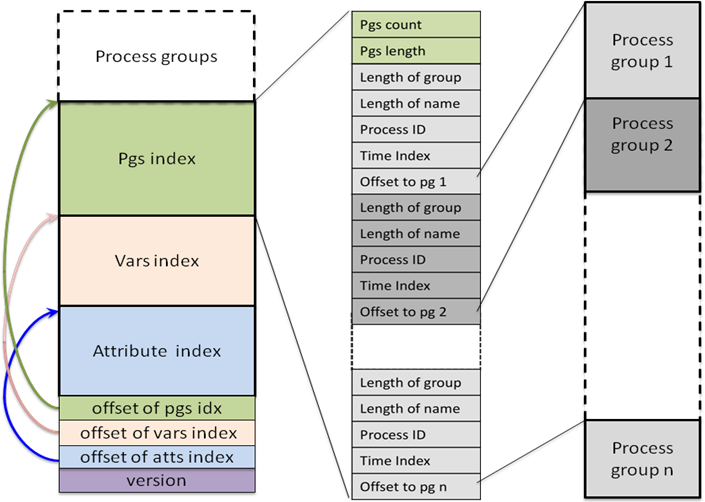
\includegraphics[width=338pt, height=238pt]{figures/group-index-table.png}
\caption{Group index table}
\label{fig:group-index-table}
\end{center}
\end{figure}

\subsubsection{Variables index table}

The variables index table is composed of the total count of variables in the BP 
file, the size of variables index table, and a list of variable records. Each record 
contains the size of the record and the basic metadata to describe the variable. 
As shown in Figure \ref{fig:variables-index-table}, 
the metadata include the name of the variable, the name 
of the group the variable is associated with, the data type of the variable, and 
a series of characteristic features. The structure of each characteristic entry 
contains an offset value, which is addressed to the certain occurrence of the variable 
in the BP file. For instance, if n processes write out the variable ``d'' per time 
step, and m iterations have been completed during the whole simulation, then the 
variable will be written (m\textit{ }\ensuremath{\times} n) times in the BP file 
that is produced. Accordingly, there will be the same number of elements in the 
list of characteristics. In this way, we can quickly retrieve the single dataset 
for all time steps or any other selection of time steps. This flexibility and efficiency 
also apply to a scenario in which a portion of records needs to be collected from 
a certain group of processes. 

\begin{figure}[htbp]
\begin{center}
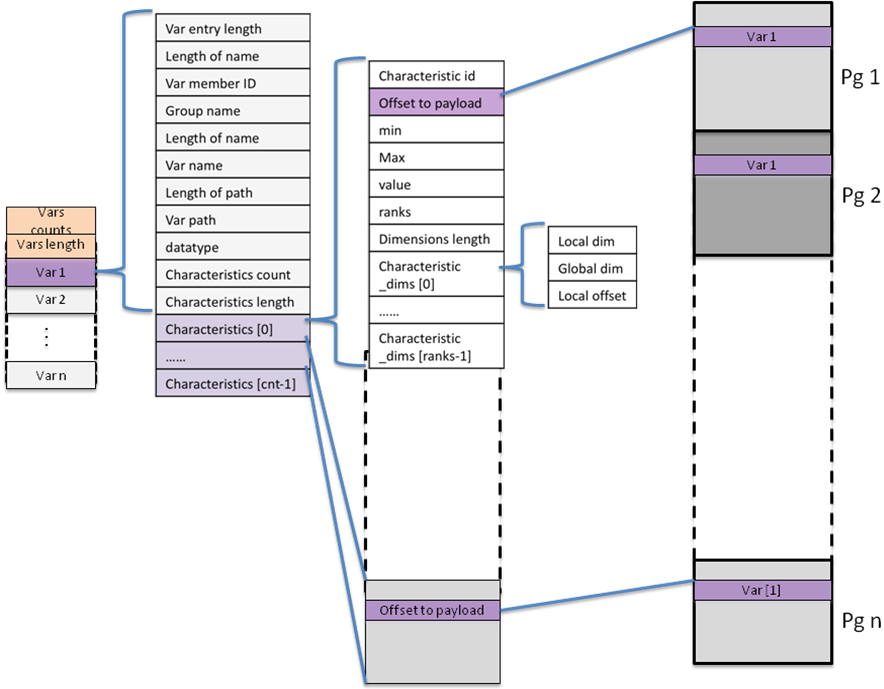
\includegraphics[width=420pt, height=327pt]{figures/variables-index-table.png}
\caption{Variables index table}
\label{fig:variables-index-table}
\end{center}
\end{figure}

\subsubsection{Attributes index table}

Since an attribute can be considered to be a special type of variable, its index 
table in BP format is organized in the same way as a variables index table and 
therefore supports the same types of features mentioned in the previous sections. 

\section{Process Groups}

One of the major concepts in BP format is what is called ``process group'' or PG. 
The BP file format encompasses a series of PG entries and the BP file footer. Each 
process group is the entire self-contained output from a single process and is 
written out independently into a contiguous disk space. In that way, we can enhance 
parallelism and reduce coordination among processes in the same communication group. 
The data diagram in Figure \ref{fig:process-group-struct} 
illustrates the detailed content in each PG. 

\begin{figure}[htbp]
\begin{center}
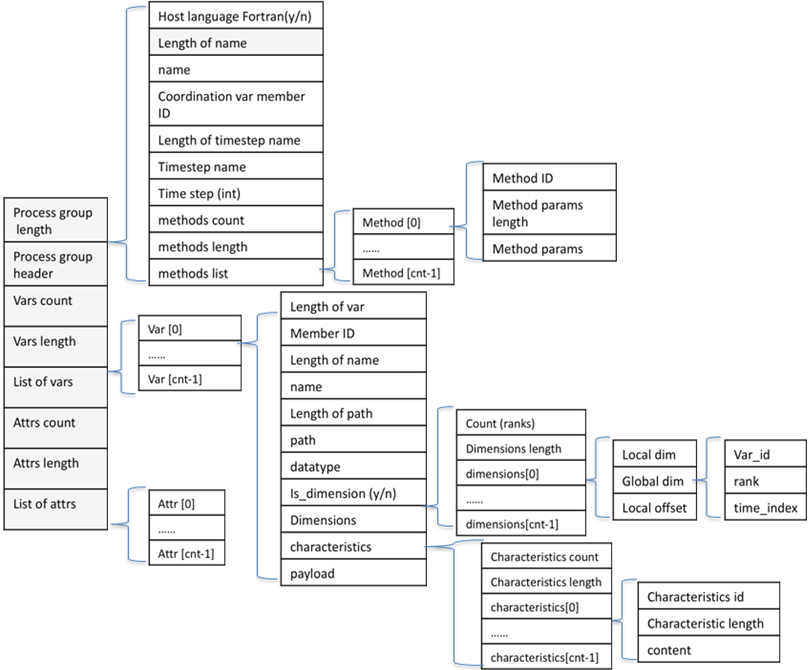
\includegraphics[width=389pt, height=321pt]{figures/process-group-structure.png}
\caption{Process group structure}
\label{fig:process-group-struct}
\end{center}
\end{figure}

\subsection{PG header}

\subsubsection{Unlimited dimension}

BP format allows users to define an unlimited dimension, which will be specified 
as the time-index in the XML file. Users can define variables having a dimension 
with undefined length, for which the variable can grow along that dimension. PG 
is a self-contained, independent data structure; the dataset in the local space 
per each time step is not reconstructed at the writing operations across the processes 
or at time steps. Theoretically, PGs can be appended to infinity; they can be added 
one after another no matter how many processes or time steps take place during 
the simulation.  Thus ADIOS is able to achieve high I/O performance.

\subsubsection{Transport methods}

One of the advantages of organizing output in terms of groups is to categorize 
all the variables based on their I/O patterns and logical relationships. It provides 
flexibility for each group to choose the optimized transport method according to 
the simulation environment and underlying hardware configuration or the transport 
methods used for a performance study without even changing the source code. In 
PG header structure, each entry in the method list has a method ID and method parameters, 
such as system-tuning parameters or underneath driver selection. 

\subsection{Vars list}

\subsubsection{Var header}

\emph{Dimensions structure.} 
Internal to bp is sufficient information to recreate any global structure and to 
place the local data into the structure. In the case of a global array, each process 
writes the size of the global array dimensions, specifies the local offsets into 
each, and then writes the local data, noting the size in each dimension. On conversion 
to another format, such as HDF5, this information is used to create hyperslabs 
for writing the data into the single, contiguous space. Otherwise, it is just read 
back in and used to note where the data came from. In this way, we can enhance 
parallelism and reduce coordination. All of our parallel writes occur independently 
unless the underlying transport specifically requires collective operations. Even 
in those cases, the collective calls are only for a full buffer write (assuming 
the transport was written appropriately) unless there is insufficient buffer space. 

As shown in Figure 19, the dimension structure contains a time index flag, which 
indicates whether this variable has an unlimited time dimension. Var\_id is used 
to retrieve the dimension value if the dimension is defined as variable in the 
XML file; otherwise, the rank value is taken as the array dimension.  

\subsubsection{Payload}

Basic statistical characteristics give users the advantage for quick data inspection 
and analysis. In Figure 19, redundant information about characteristics is stored 
along with variable payload so that if the characteristics part in the file footer 
gets corrupted, it can still be recovered quickly. Currently, only simple statistical 
traits are saved in the file, but the characteristics structure will be easily 
expanded or modified according to the requirements of scientific applications or 
the analysis tools. 

\subsection{Attributes list}

The layout of the attributes list (see Figure \ref{fig:attribute-entry-struct}) 
is very similar to that of the 
variables. However, instead of containing dimensional structures and physical data 
load, the attribute header has an is\_var flag, which indicates either that the 
value of the attribute is referenced from a variable by looking up the var\_id 
in the same group or that it is a static value defined in the XML file. 

\begin{figure}[htbp]
\begin{center}
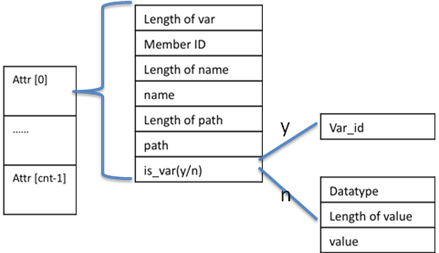
\includegraphics[width=210pt, height=120pt]{figures/attributes-entry-structure.png}
\caption{Attribute entry structure}
\label{fig:attribute-entry-struct}
\end{center}
\end{figure}



\chapter{Developer Manual}

\section{Create New Transport Methods}

One of ADIOS's important features is the componentization of transport methods. 
Users can switch among the typical methods that we support or even create their 
own methods, which can be easily plugged into our library. The following sections 
provide the procedures for adding the new transport method called ``abc'' into 
the ADIOS library. In this version of ADIOS, all the source files are located in 
/trunk/src/; the core files in /trunk/src/core/, the write method in /trunk/src/write
and the read method in /trunk/src/read.

\subsection{Add the new method macros in adios\_transport\_hooks.h}

The first file users need to examine is adios\_transport\_hooks.h, which basically 
defines all the transport methods and interface functions between detailed transport 
implementation and user APIs. In the file, we first find the line that defines 
the enumeration type Adios\_IO\_methods\_datatype add the declaration of method 
ID ADIOS\_METHOD\_ABC, and, because we add a new method, update total number of 
transport methods ADIOS\_METHOD\_COUNT from 9 to 10.

1. enum Adios\_IO\_methods datatype 
\begin{lstlisting}[caption={Add a new write method, step 1}]

enum ADIOS_IO_METHOD {
    ADIOS_METHOD_UNKNOWN    = -2,
    ADIOS_METHOD_NULL       = -1,
    ADIOS_METHOD_MPI        = 0,
    ...
    ADIOS_METHOD_PROVENANCE = 8,

    `\color{javapurple}{\bf ADIOS\_METHOD\_ABC        = 9,}`

    ADIOS_METHOD_COUNT      = 10
};
\end{lstlisting}

2. Next, we need to declare the transport APIs for method ``abc,'' including init/finalize, 
open/close, should\_buffer, and read/write. Similar to the other methods, we need 
to add 

\begin{lstlisting}
    FORWARD_DECLARE (abc)
\end{lstlisting}

3. Then, we add the mapping of the string name ``abc'' of the new transport method 
to the method ID - ADIOS\_METHOD\_ABC, which has been already defined in enumeration 
type Adios\_IO\_methods\_datatype. As the last parameter, ``1'' here means the 
method requires communications, or ``0'' if not.

\begin{lstlisting}
    MATCH_STRING_TO_METHOD ("abc", ADIOS_METHOD_ABC, 1)     
\end{lstlisting}
        
4. Lastly, we add the mapping of the string name needed in the initialization functions 
to the method ID, which will be used by adios\_transport\_struct variables defined 
in adios\_internals.h.

\begin{lstlisting}
    ASSIGN_FNS (abc, ADIOS_METHOD_ABC)
\end{lstlisting}

\subsection{Create adios\_abc.c}

In this section, we demonstrate how to implement different transport APIs for method 
``abc.'' In adios\_abc.c, we need to implement at least 11 required routines: 

\begin{enumerate}
\item ``adios\_abc\_init'' allocates the method\_data field in adios\_method\_struct 
to the user-defined transport data structure, such as adios\_abc\_data\_struct, 
and initializes this data structure. Before the function returns, the initialization 
status can be set by statement ``adios\_abc\_initialized = 1.''

\item ``adios\_abc\_open'' opens a file if there is only one processor writing to 
the file. Otherwise, this function does nothing; instead, we use adios\_abc\_should\_buffer 
to coordinate the file open operations.   

\item ``adios\_abc\_should\_buffer,'' called by the ``common\_adios\_group\_size'' 
function in adios.c, needs to include coordination of open operations if multiple 
processes are writing to the same file. 

\item ``adios\_abc\_write'', in the case of no buffering or overflow, writes data 
directly to disk. Otherwise, it verifies whether the internally recorded memory 
pointer is consistent with the vector variable's address passed in the function 
parameter and frees that block of memory if it is not needed any more.  

\item ``adios\_abc\_read'' associates the internal data structure's address to the 
variable specified in the function parameter.

\item ``adios\_abc\_close'' simply closes the file if no buffering scheme is used. 
However, in general, this function performs most of the actual disk writing/reading 
the buffers to/from the file by one or more processors in the same communicator 
domain and then close the file. 

\item ``adios\_abc\_finalize'' resets the initialization status back to 0 if it has 
been set to 1 by adios\_abc\_init. 

If you are developing asynchronous methods, the following functions need to be 
implemented as well; otherwise you can leave them as empty implementation.

\item adios\_abc\_get\_write\_buffer,

\item ``adios\_abc\_end\_iteration`` is a tick counter for the I/O 
routines to time how fast they are emptying the buffers. 

\item ``adios\_abc\_start\_calculation'' indicates that it is now 
an ideal time to do bulk data transfers because the code will not be performing 
I/O for a while.

\item ``adios\_abc\_stop\_calculation`` indicates that bulk data 
transfers should cease because the code is about to start communicating with other 
nodes.
\end{enumerate}

The following is One of the most important things that needs to be noted: 

fd-\texttt{>}shared\_buffer = adios\_flag\_no,

which means that the methods do not need a buffering scheme, such as PHDF5, and 
that data write out occurs immediately once adios\_write returns.

If fd-\texttt{>}shared\_buffer = adios\_flag\_yes, the users can employ the self-defined 
buffering scheme to improve I/O performance.

\subsection{A walk-through example}

Now let's look at an example of adding an unbuffered POSIX method to ADIOS.  According 
to the steps described above, we first open the header file --``adios\_transport\_hooks.h,'' 
and add the following statements:

\begin{lstlisting}[emph={ADIOS_METHOD_POSIX_ASCII_NB}, emphstyle={\color{red}\large\bf},
                   caption={Example: add unbuffered POSIX method, step 1}]
enum ADIOS_IO_METHOD {

    ADIOS_METHOD_UNKNOWN        = -2,
    ADIOS_METHOD_NULL           = -1,
    ADIOS_METHOD_MPI            = 0,
    ...
    ADIOS_METHOD_PROVENANCE     = 8,
    // method ID for binary transport method
    ADIOS_METHOD_POSIX_ASCII_NB = 9, 
    // total method number
    ADIOS_METHOD_COUNT          = 10 
};

FORWARD_DECLARE (posix_ascii_nb);

MATCH_STRING_TO_METHOD ("posix_ascii_nb", ADIOS_METHOD_POSIX_ASCII_NB, 0)

ASSIGN_FNS (binary, ADIOS_METHOD_POSIX_ASCII_NB)
\end{lstlisting}

Next, we must create adios\_posix\_ascii\_nb,c, which defines all the required 
routines listed in Sect. 12.1.2 The blue highlights below mark out the data structures 
and required functions that developers need to implement in the source code. 

\begin{lstlisting}[emph={ADIOS_METHOD_POSIX_ASCII_NB}, emphstyle={\color{red}\large\bf},
                   caption={Example: add unbuffered POSIX method, C source of write method}]
static int adios_posix_ascii_nb_initialized = 0;

struct adios_POSIX_ASCII_UNBUFFERED_data_struct
{
    FILE *f;
    uint64_t file_size;
};

void adios_posix_ascii_nb_init (const char *parameters, 
                                struct adios_method_struct * method)
{
    struct adios_POSIX_ASCII_UNBUFFERED_data_struct * md;

    if (!adios_posix_ascii_nb_initialized)
    {
        adios_posix_ascii_nb_initialized = 1;
    }

    method->method_data = malloc (
            sizeof(struct adios_POSIX_ASCII_UNBUFFERED_data_struct));
    md = (struct adios_POSIX_ASCII_UNBUFFERED_data_struct *) 
            method->method_data;
    md->f = 0;
    md->file_size = 0;
}

int adios_posix_ascii_nb _open (struct adios_file_struct * fd, 
                                struct adios_method_struct * method)
{
    char * name;
    struct adios_POSIX_ASCII_UNBUFFERED_data_struct * p;
    struct stat s;

    p = (struct adios_POSIX_ASCII_UNBUFFERED_data_struct *) 
            method->method_data;
    name = malloc (strlen (method->base_path) + strlen (fd->name) + 1);
    sprintf (name, "\%s\%s", method->base_path, fd->name);
    if (stat (name, \&s) == 0)
        p->file_size = s.st_size;

    switch (fd->mode)
    {
        case adios_mode_read:
        {
            p->f = fopen (name, "r");
            if (p->f <= 0)
            {
                fprintf (stderr, "ADIOS POSIX ASCII UNBUFFERED: "
                        "file not found: \%s\n", fd->name);
                free (name);
                return 0;
            }
            break;
        }

        case adios_mode_write:
        {
            p->f = fopen (name, "w");
            if (p->f <= 0)
            {
                fprintf (stderr, "adios_posix_ascii_nb_open " 
                        "failed for base_path %s, name %s\n", 
                        method->base_path, fd->name 
                        );
                free (name);
                return 0;
            }
            break;
        } 

        case adios_mode_append:
        {
            int old_file = 1;
            p->f = fopen (name, "a");
            if (p->f <= 0)
            {
                fprintf (stderr, "adios_posix_ascii_nb_open"
                        " failed for base_path \%s, name \%s\n"
                        ,method->base_path, fd->name
                        );
                free (name);
                return 0;
            }
            break;
        }

        default:
        {
            fprintf (stderr, "Unknown file mode: \%d\n", fd->mode);
            free (name);
            return 0;
        }
    }
    free (name);
    return 0;
}

enum ADIOS_FLAG adios_posix_ascii_nb_should_buffer(
                            struct adios_file_struct * fd,
                            struct adios_method_struct * method,
                            void * comm) 
{
    //in this case, we don't use shared_buffer
    return adios_flag_no;
}

void adios_posix_ascii_nb_write (struct adios_file_struct * fd,
                                 struct adios_var_struct * v,
                                 void * data,
                                 struct adios_method_struct * method) 
{
    struct adios_POSIX_ASCII_UNBUFFERED_data_struct * p;
    p = (struct adios_POSIX_ASCII_UNBUFFERED_data_struct *)
            method->method_data;
    if (!v->dimensions) {
        switch (v->type)
        {
            case adios_byte:
            case adios_unsigned_byte:
                fprintf (p->f,"\%c\n", *((char *)data)); 
                break;
            case adios_short:
            case adios_integer:
            case adios_unsigned_short:
            case adios_unsigned_integer:
                fprintf (p->f,"\%d\n", *((int *)data)); 
                break;
            case adios_real:
            case adios_double:
            case adios_long_double:
                fprintf (p->f,"\%f\n", *((double *)data)); 
                break;
            case adios_string:
                fprintf (p->f,"\%s\n", (char *)data); 
                break;
            case adios_complex:
                fprintf (p->f,"\%f+\%fi\n", 
                         *((float *)data),*((float *)(data+4))); 
                break;
            case adios_double_complex:
                fprintf (p->f,"\%f+\%fi\n", 
                         *((double *)data),*((double *)(data+8))); 
                break;
            default:
                break;
        }
    } 
    else
    {
        uint64_t j;
        int element_size = adios_get_type_size (v->type, v->data);
        printf("element_size: \%d\n",element_size);
        uint64_t var_size = adios_get_var_size (v, fd->group, v->data) /
                                element_size;
        switch (v->type)
        {
            case adios_byte:
            case adios_unsigned_byte:
                for (j = 0;j < var_size; j++)
                    fprintf (p->f,"\%c ", *((char *)(data+j)));
                printf("\n");
                break;
            case adios_short:
            case adios_integer:
            case adios_unsigned_short:
            case adios_unsigned_integer:
                for (j = 0;j < var_size; j++)
                    fprintf (p->f,"\%d ", *((int *)(data+element_size*j)));
                printf("\n");
                break;
            case adios_real:
            case adios_double:
            case adios_long_double:
                for (j = 0;j < var_size; j++)
                    fprintf (p->f,"\%f ", * ( (double *)(data+element_size*j)));
                printf("\n");
                break;
            case adios_string:
                for (j = 0;j < var_size; j++)
                    fprintf (p->f,"\%s ", (char *)data);
                printf("\n");
                break;
            case adios_complex:
                for (j = 0;j < var_size; j++)
                    fprintf (p->f, "\%f+\%fi ", *((float *)(data+element_size*j)),
                            *((float *)(data+4+element_size*j)));
                printf("\n");
                break;
            case adios_double_complex:
                for (j = 0;j < var_size; j++)
                    fprintf (p->f,"\%f+\%fi ", *((double *)(data+element_size*j)),
                            *((double *)(data+element_size*j+8)));
                printf("\n");
                break;
            default:
                break;
        } 
    }
}

void adios_posix_ascii_nb_get_write_buffer (struct adios_file_struct * fd,
                                            struct adios_var_struct * v,
                                            uint64_t * size,
                                            void ** buffer,
                                            struct adios_method_struct * method)
{
*buffer = 0;
}

void adios_posix_ascii_nb_read (struct adios_file_struct * fd,
                                struct adios_var_struct * v, 
                                void * buffer,
                                uint64_t buffer_size,
                                struct adios_method_struct * method)
{
    v->data = buffer;
    v->data_size = buffer_size; 
}

int adios_posix_ascii_nb_close (struct adios_file_struct * fd,
                                struct adios_method_struct * method)
{
    struct adios_POSIX_ASCII_UNBUFFERED_data_struct * p;
    p = (struct adios_POSIX_ASCII_UNBUFFERED_data_struct *)
        method->method_data;
    if (p->f <= 0)
    {
        fclose (p->f);
    }
    p->f = 0;
    p->file_size = 0; 
}

void adios_posix_ascii_nb_finalize (int mype, 
                                    struct adios_method_struct * method)} 
{
    if (adios_posix_ascii_nb_initialized)
        adios_posix_ascii_nb_initialized = 0; 
}

\end{lstlisting}

The binary transport method blocks methods for simplicity. Therefore,  no special 
implementation for the three functions below is necessary and their function bodies 
can be left empty:

\begin{lstlisting}
adios_posix_ascii_nb_end_iteration (struct adios_method_struct * method) {}
adios_posix_ascii_nb_start_calculation (struct adios_method_struct * method) {}
adios posix_ascii_nb stop_calculation (struct adios_method_struct * method) {}
\end{lstlisting}

Above, we have implemented the POSIX\_ASCII\_NB transport method. When users specify 
POSIX\_ASCII\_NB method in xml file, the users' applications will generate ASCII 
files by using common ADIOS APIs. However, in order to achieve better I/O performance, 
a buffering scheme needs to be included into this example.

\section{Profiling the Application and ADIOS}

There are two ways to get profiling information of ADIOS I/O operations. One way 
is for the user to explicitly insert a set of profiling API calls around ADIOS 
API calls in the source code. The other way is to link the user code with a renamed 
ADIOS library and an ADIOS API wrapper library. 

\subsection{Use profiling API in source code}

The profiling library called libadios\_timing.a implements a set of profiling API 
calls. The user can use these API calls to wrap the ADIOS API calls in the source 
code to get profiling information. 

The adios-timing.h header file contains the declarations of those profiling functions. 

\begin{lstlisting}[frame=single, backgroundcolor=\color{gray85}]
/*
 * initialize profiling 
 *
 * Fortran interface
 */
int init_prof_all_(char *prof_file_name, int prof_file_name_size);

/*
 * record open start time for specified group
 *
 * Fortran interface
 */
void open_start_for_group_ (int64_t *gp_prof_handle, char *group_name, 
                            int *cycle, int *gp_name_size);

/*
 * record open end time for specified group
 *
 * Fortran interface
 */
void open_end_for_group_(int64_t *gp_prof_handle, int *cycle);

/*
 * record write start time for specified group
 *
 * Fortran interface
 */
void write_start_for_group_(int64_t *gp_prof_handle, int *cycle);

/*
 * record write end time for specified group
 *
 * Fortran interface
 */
void write_end_for_group_(int64_t *gp_prof_handle, int *cycle);

/*
 * record close start time for specified group
*
 * Fortran interface
 */
void close_start_for_group_(int64_t *gp_prof_handle, int *cycle);

/*
 * record close end time for specified group
 *
 * Fortran interface
 */
void close_end_for_group_(int64_t *gp_prof_handle, int *cycle);

/*
 * Report timing info for all groups
 *
 * Fortran interface  
 */
int finalize_prof_all_();

/*
 * record start time of a simulation cycle
 *
 * Fortran interface 
 */
void cycle_start_(int *cycle);

/*
 * record end time of a simulation cycle
 *
 * Fortran interface 
 */
void cycle_end_(int *cycle);

\end{lstlisting}

An example of using these functions is given below....

\begin{lstlisting}[language=Fortran, frame=single, backgroundcolor=\color{gray85}]
...
! initialization ADIOS
CALL adios_init ("config.xml"//char(0))
! initialize profiling library; the parameter specifies the file where 
! profiling information is written
CALL init_prof_all("log"//char(0))
...
CALL MPI_Barrier(toroidal_comm, error )
! record start time of open
! group_prof_handle is an OUT parameter holding the handle for the 
! group 'output3d.0'
! istep is iteration no.
CALL open_start_for_group(group_prof_handle, "output3d.0"//char(0),istep)

CALL adios_open(adios_handle, "output3d.0"//char(0), "w"//char(0))

! record end time of open
CALL open_end_for_group(group_prof_handle,istep)

! record start time of write
CALL write_start_for_group(group_prof_handle,istep)

#include "gwrite_output3d.0.fh"

! record end time of write
CALL write_end_for_group(group_prof_handle,istep)

! record start time of close
CALL cose_start_for_group(group_prof_handle,istep)

CALL adios_close(adios_handle,adios_err)

! record end time of close
CALL close_end_for_group(group_prof_handle,istep)

...
CALL adios_finalize (myid)

! finalize; profiling information are gathered and 
! min/max/mean/var are calculated for each IO dump
CALL finalize_prof()

CALL MPI_FINALIZE(error)


\end{lstlisting}

When the code is run, profiling information will be saved to the file ''./log'' 
(specified in init\_prof\_all ()). Below is an example.

{\small 
\begin{lstlisting}[language=Fortran, frame=single, backgroundcolor=\color{gray85}]
Fri Aug 22 15:42:04 EDT 2008
I/O Timing results
Operations   : min                 max                 mean                var
cycle no       3
io count       0
# Open       : 0.107671            0.108245            0.108032            0.000124
# Open start : 1219434228.866144   1219434230.775268   1219434229.748614   0.588501
# Open end   : 1219434228.974225   1219434230.883335   1219434229.856646   0.588486
# Write      : 0.000170            0.000190            0.000179            0.000005
# Write start: 1219434228.974226   1219434230.883336   1219434229.856647   0.588486
# Write end  : 1219434228.974405   1219434230.883514   1219434229.856826   0.588484
# Close      : 0.001608            0.001743            0.001656            0.000036
# Close start: 1219434228.974405   1219434230.883514   1219434229.856826   0.588484
# Close end  : 1219434228.976040   1219434230.885211   1219434229.858482   0.588489
# Total      : 0.109484            0.110049            0.109868            0.000137
cycle no       6
io count       1
# Open       : 0.000007            0.000011            0.000009            0.000001
# Open start : 1219434240.098444   1219434242.007951   1219434240.981075   0.588556
# Open end   : 1219434240.098452   1219434242.007962   1219434240.981083   0.588556
# Write      : 0.000175            0.000196            0.000180            0.000004
# Write start: 1219434240.098452   1219434242.007962   1219434240.981083   0.588557
# Write end  : 1219434240.098631   1219434242.008158   1219434240.981264   0.588558
# Close      : 0.000947            0.003603            0.001234            0.000466
# Close start: 1219434240.098631   1219434242.008158   1219434240.981264   0.588558
# Close end  : 1219434240.099665   1219434242.009620   1219434240.982498   0.588447
# Total      : 0.001132            0.003789            0.001423            0.000466

\end{lstlisting}
}

The script ``post\_script.sh'' extracts ``open time'', ``write time'', ``close 
time'', and ``total time'' from the raw profiling results and saves them in separate 
files: open, write, close, and total, respectively.

To compile the code, one should link the code with the -\textit{ladios\_timing 
-ladios} option. 

\subsection{Use wrapper library}

Another way to do profiling is to link the source code with a renamed ADIOS library 
and a wrapper library. 

The renamed ADIOS library implements ``real'' ADIOS routines, but all ADIOS public 
functions are renamed with a prefix ``P''. For example, adios\_open() is renamed 
as Padios\_open(). The routine for parsing config.xml file is also changed to parse 
extra flags in config.xml file to turn profiling on or off.

The wrapper library implements all adios pubic functions (e.g., adios\_open, adios\_write, 
adios\_close) within each function. It calls the ``real'' function (Padios\_xxx()) 
and measure the start and end time of the function call. 

There is an example wrapper library called libadios\_profiling.a. Developers can 
implement their own wrapper library to customize the profiling.

To use the wrapper library, the user code should be linked with -\textit{ladios\_profiling 
-ladios}. the wrapper library should precede the ``real'' ADIOS library. There 
is no need to put additional profiling API calls in the source code. The user can 
turn profiling on or off for each ADIOS group by setting a flag in the config.xml 
file.

\begin{lstlisting}
<adios-group name="restart.model" profiling="yes|no">
    ...
</adios-group\>
\end{lstlisting}


\chapter{Appendix}
\label{section-appendix}




\end{document}





